% PUMA TPC reconstruction — curated slide set (build up section by section)
% Compile: tectonic PUMA_slides.tex   (figures in ./figs/)
\documentclass[aspectratio=169,11pt]{beamer}
\usetheme{Madrid}\usecolortheme{whale}
\usepackage{graphicx,booktabs}
\setbeamertemplate{navigation symbols}{}
\setbeamertemplate{footline}[frame number]
\setbeamercolor{frametitle}{bg=structure!85!black}

\title[PUMA TPC reconstruction]{PUMA TPC --- track reconstruction}
\subtitle{Event representation, pulse analysis, tracking}
\date{}

\begin{document}
\frame{\titlepage}

\section{Event representation}

\begin{frame}{The PUMA active volume}
\begin{columns}
\column{0.5\textwidth}
\begin{itemize}
\item Annular gas TPC: \textbf{P10 @ 1 bar}, R = 62.9--121.1 mm, drift length 300 mm, \textbf{B = 4 T} solenoid.
\item Pad plane: \textbf{16 equal-area rings $\times$ 256 azimuthal pads} = 4096 pads.
\item A charged track ionises the gas $\to$ electrons drift to the pads.
\item Each pad gives \((x,y)\) from its position and \(z\) from the \textbf{drift time} of the pulse.
\end{itemize}
\column{0.5\textwidth}
\centering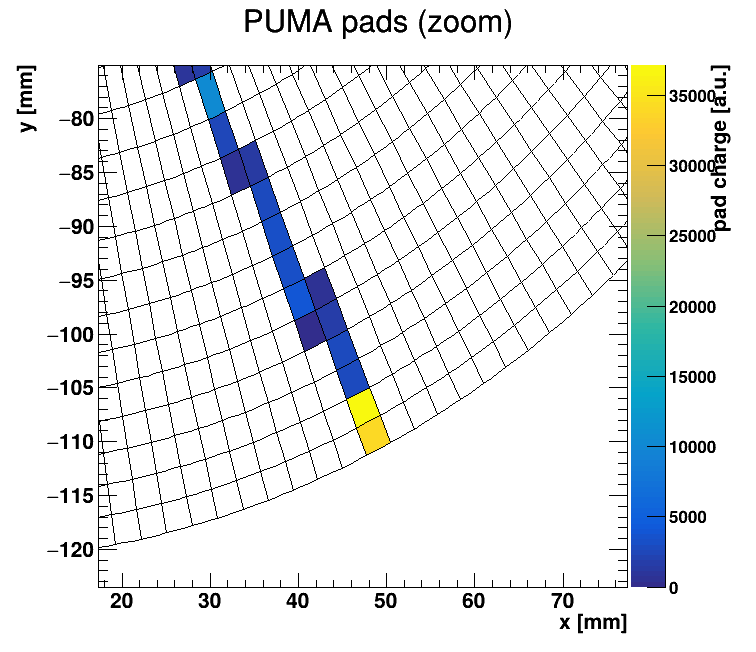
\includegraphics[width=\linewidth]{figs/pad_zoom.png}\\
{\scriptsize A track fires a column of pads; colour = charge.}
\end{columns}
\end{frame}

\begin{frame}{A reconstructed event --- 2D pad plane}
\centering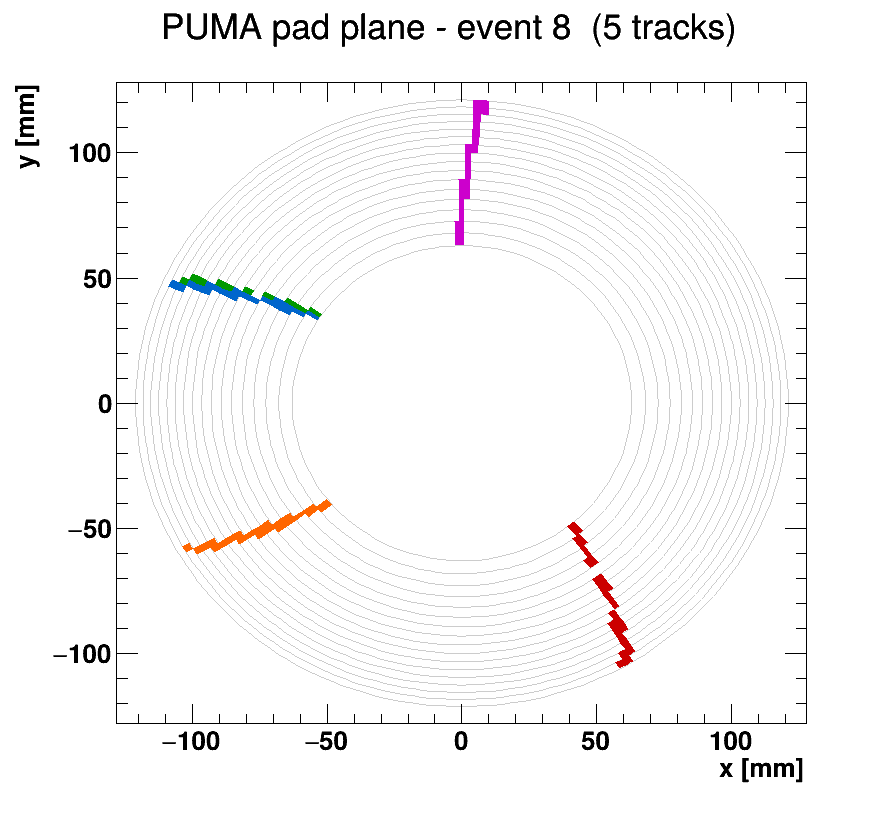
\includegraphics[height=.74\textheight]{figs/track_2d.png}\\
{\small Each fired pad drawn as its real annular sector, coloured by the pattern-recognition track it belongs to. Five tracks; the concentric circles are the 16 ring boundaries.}
\end{frame}

\begin{frame}{The same event --- in 3D}
\centering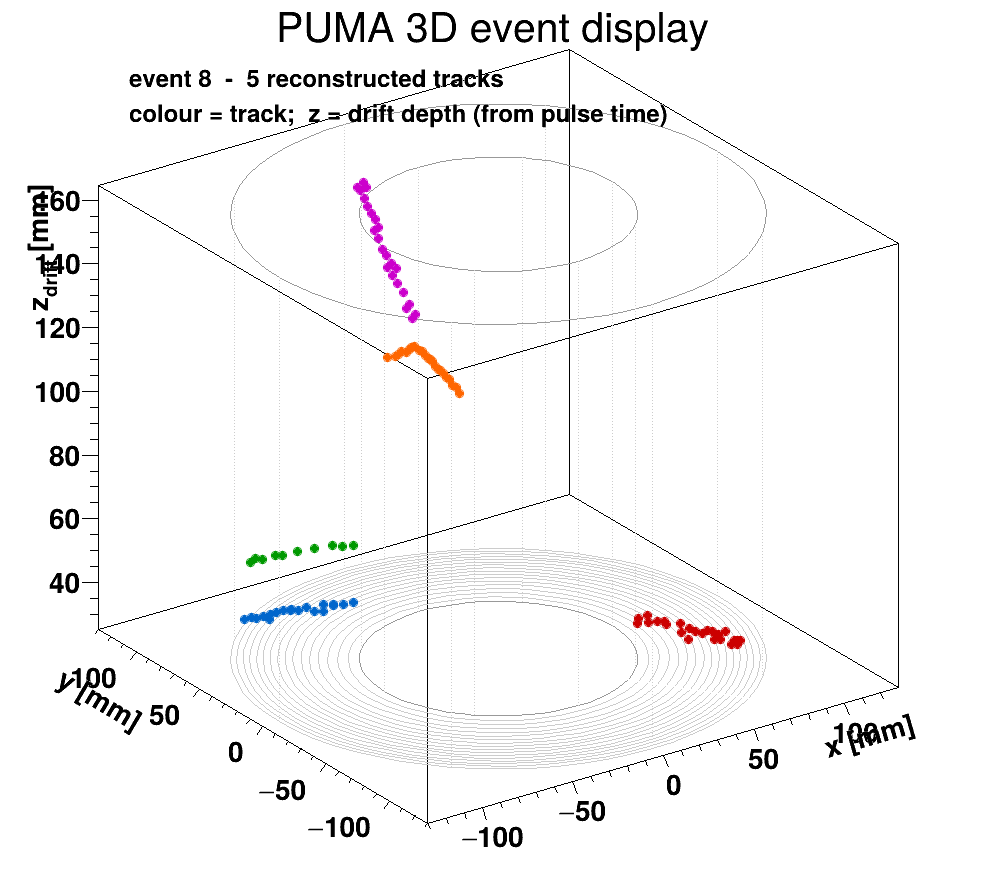
\includegraphics[height=.74\textheight]{figs/track_3d.png}\\
{\small Same five tracks in \((x,y,z_{\mathrm{drift}})\): the pad gives \((x,y)\), the pulse arrival time gives \(z\). Tracks sit at different drift depths inside the annular TPC volume.}
\end{frame}

\section{Pulse-shape analysis}

\begin{frame}[fragile]{From pad pulses to hits --- the PSA fit}
\centering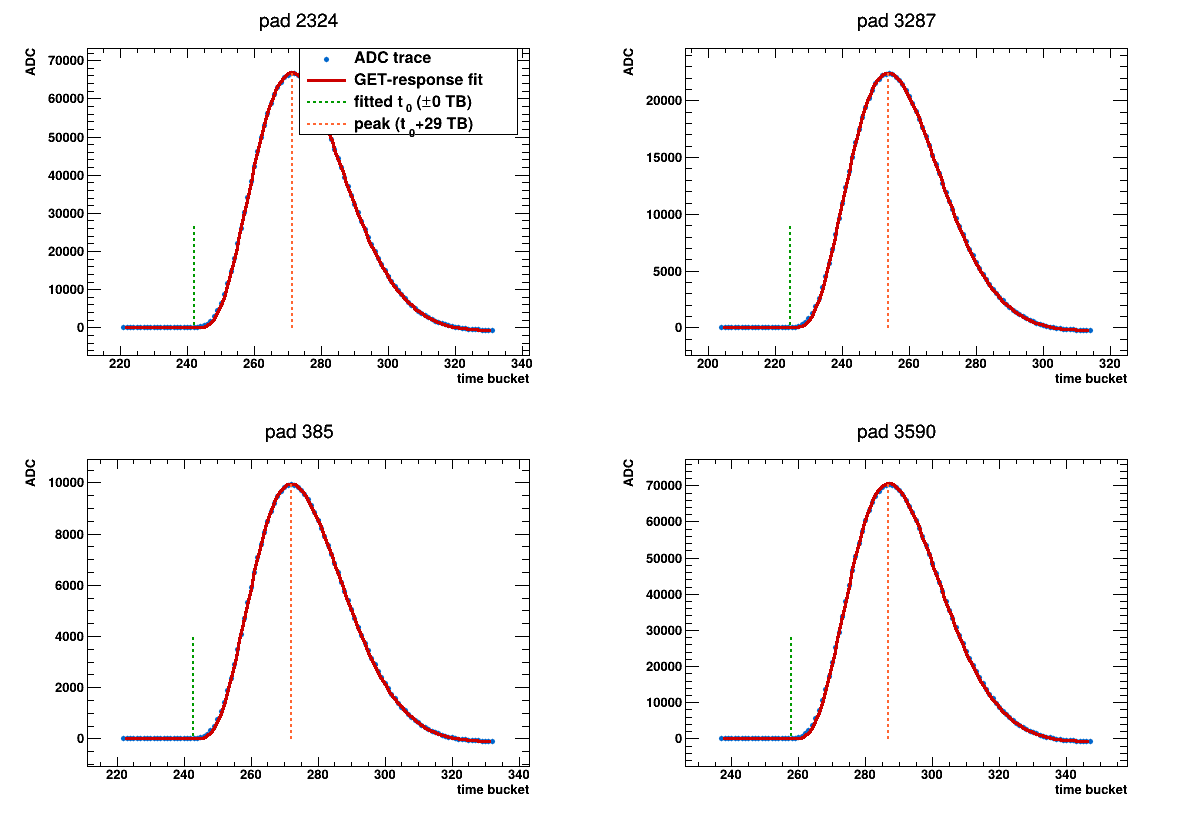
\includegraphics[height=.62\textheight]{figs/psa_fitshape.png}\\
{\small Pad ADC traces (blue) with the \textbf{GET electronics-response fit} (red, \texttt{AtPSAMultiFit}: \(A\,e^{-3u}\sin u\,u^3\), \(u=(t-t_0)/\tau\), \(\tau=25\) TB) --- overlays the pulse shape \textbf{perfectly}. The fitted \textcolor{green!60!black}{impulse time \(t_0\)} gives the \textbf{unbiased} drift depth (\(z\)); the \textcolor{orange}{response peak} lags \(t_0\) by the \(\sim\)8.6 mm shaping delay. One fitted pulse \(\to\) one \texttt{AtHit}.}
\end{frame}

\section{Pattern recognition}

\begin{frame}{Finding tracks: cluster first, then fit}
\begin{columns}
\column{0.52\textwidth}
\centering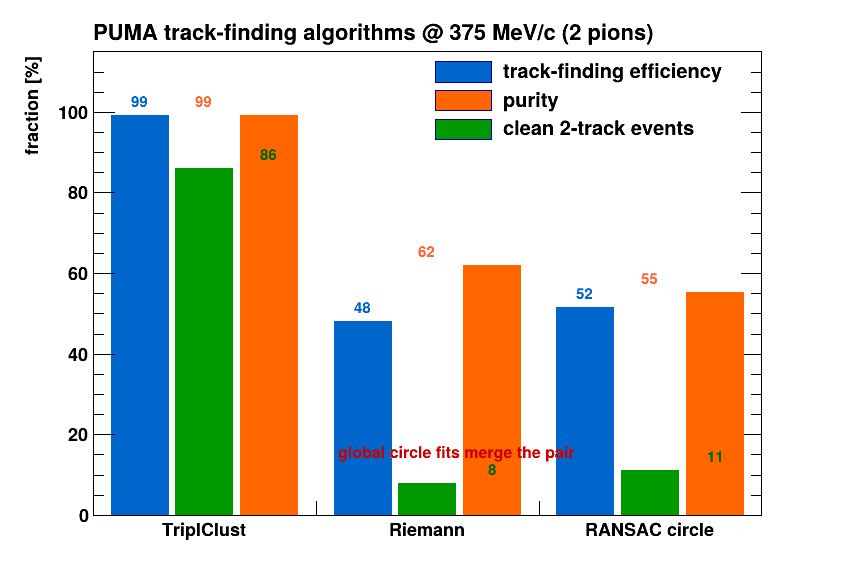
\includegraphics[width=\linewidth]{figs/pra_algo_cmp.png}
\column{0.48\textwidth}
Pattern recognition groups the \texttt{AtHit}s into tracks. Two paradigms:
\begin{itemize}
\item \textbf{spatial clustering} --- TriplClust, HDBSCAN
\item \textbf{global circle consensus} --- Riemann, RANSAC
\end{itemize}
On the 2-pion channel at 375 MeV/c, \textbf{clustering finds both tracks} (99\% eff, 99\% purity, 86\% clean events). The global circle fits fit \emph{one} dominant circle and \alert{merge the back-to-back pair} ($\sim$50\% eff, $\sim$10\% clean).\\[.4em]
\textbf{Lesson:} cluster the hits first, then fit each track --- don't fit one global circle to a multi-track event.
\end{columns}
\end{frame}

\begin{frame}{Track-finding efficiency vs momentum}
\centering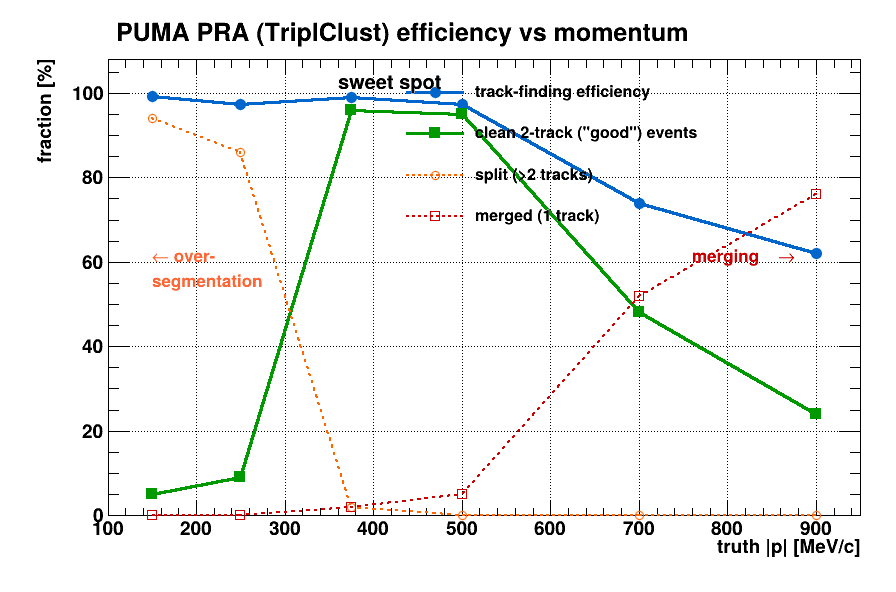
\includegraphics[height=.66\textheight]{figs/pra_eff_vs_p.png}\\
{\small Truth-matched efficiency \& clean-2-track fraction (TriplClust). \textbf{Sweet spot 375--500 MeV/c} (95\% clean --- the PUMA pion range). Two failure modes: \textcolor{orange}{over-segmentation} at low \(p\) (tight curls fragment into $>$2 tracks) and \textcolor{red}{merging} at high \(p\) (near-straight tracks fuse). Efficiency stays high; \emph{event quality} degrades at both ends.}
\end{frame}

\begin{frame}{HDBSCAN vs TriplClust --- robustness at high \(p\)}
\begin{columns}
\column{0.56\textwidth}
\centering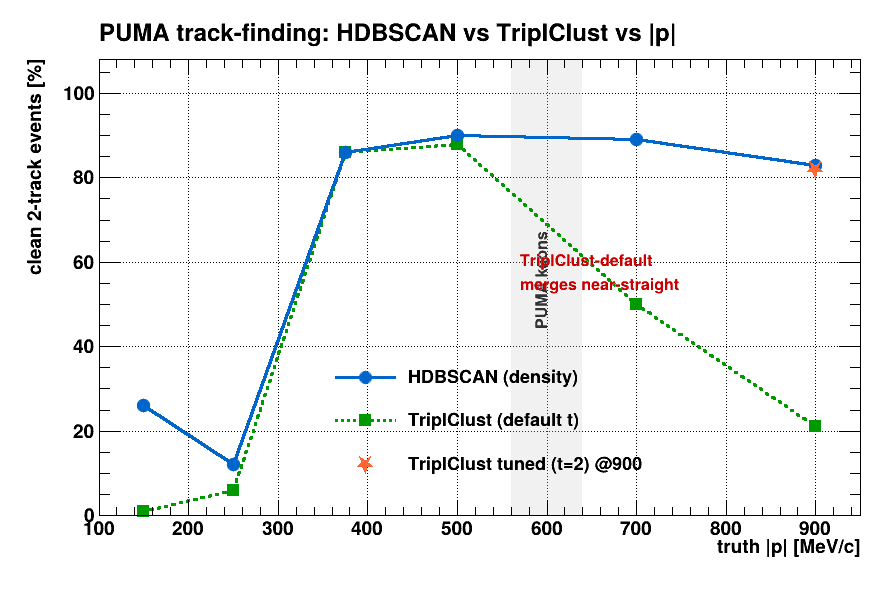
\includegraphics[width=\linewidth]{figs/pra_algo_vs_p.png}
\column{0.44\textwidth}
Same reco, two clustering finders:
\begin{itemize}
\item \textbf{HDBSCAN} (density) holds \textbf{83--90\%} clean events from 375--900 MeV/c --- it does \emph{not} merge near-straight tracks.
\item \textbf{TriplClust} (default \(t\)) matches it in the sweet spot but \alert{collapses above 500} MeV/c.
\end{itemize}
Crucial for the \textbf{PUMA kaons} ($\sim$600 MeV/c, high-\(p\)). TriplClust \emph{can} recover with a lowered cluster distance (\(t=2\) @900 $\to$ 82\%, \textcolor{orange}{$\star$}) --- but needs momentum-adaptive tuning.\\[.3em]
\textbf{Recommendation:} HDBSCAN as the default track finder (or adaptive-\(t\) TriplClust).
\end{columns}
\end{frame}

\begin{frame}{The decisive case: same-charge K\(^+\)K\(^+\)}
\begin{columns}
\column{0.54\textwidth}
\centering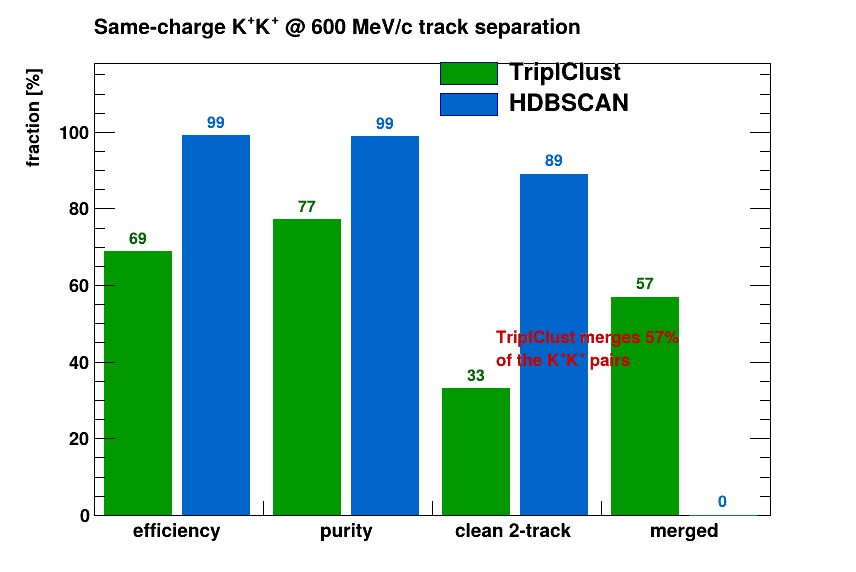
\includegraphics[width=\linewidth]{figs/pra_kaon_cmp.png}
\column{0.46\textwidth}
The real PUMA target: \(^3\)He\,+\,\(\bar p \to\) K\(^+\)K\(^+\)\(\pi^-\). The two kaons are \textbf{same charge} (mirror circles) and \textbf{near-straight} at 600 MeV/c --- the worst case for track separation.\\[.5em]
\textbf{TriplClust merges 57\%} of the pairs (33\% clean events). \textbf{HDBSCAN separates them cleanly} --- 99\% efficiency, 99\% purity, \textbf{89\% clean events, 0\% merged}.\\[.5em]
This is the case that decides the track finder: \alert{HDBSCAN for PUMA}.
\end{columns}
\end{frame}

\begin{frame}{Pattern recognition --- examples}
\centering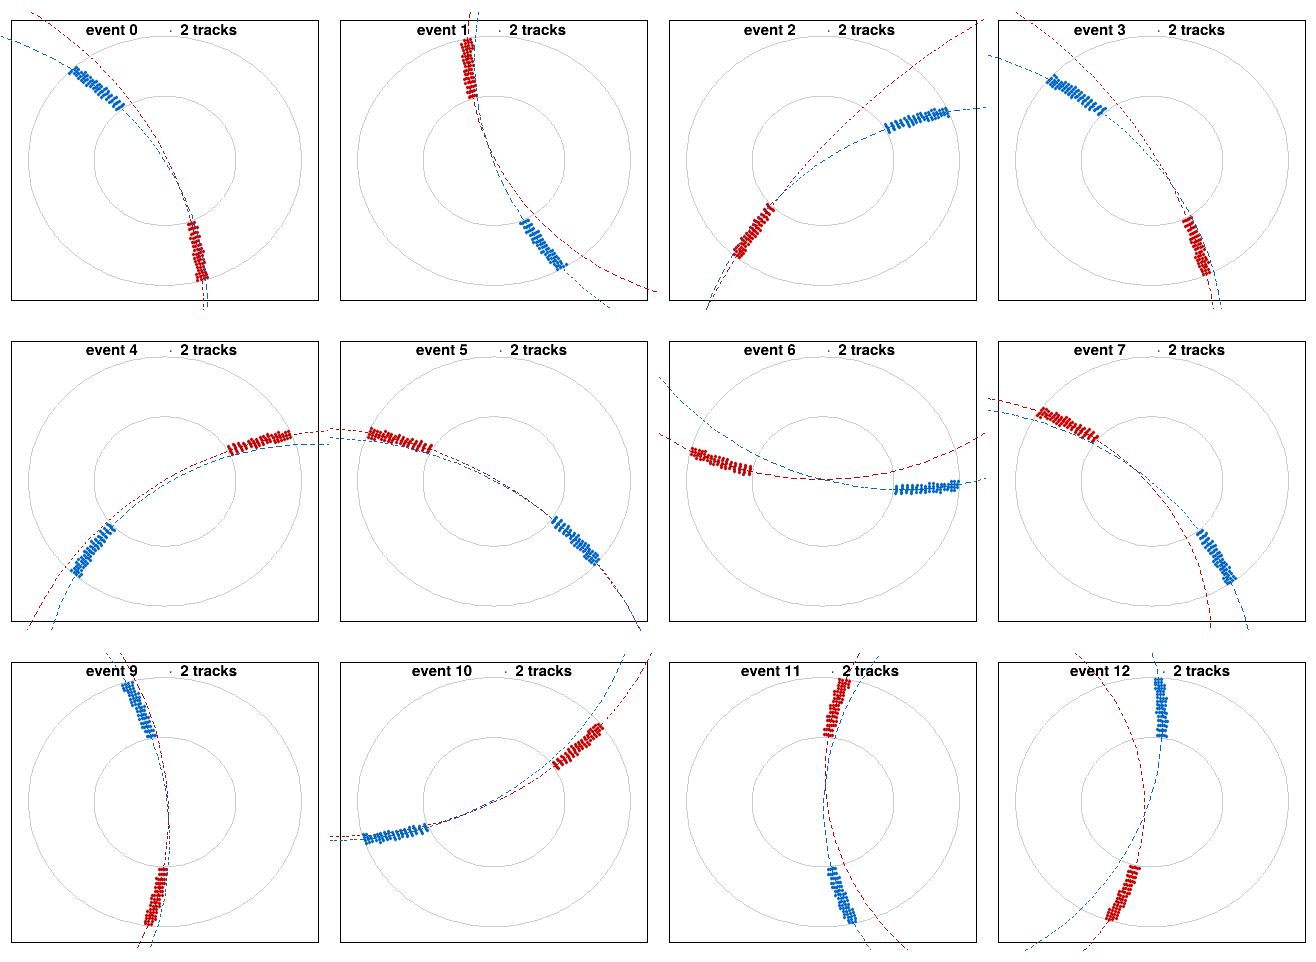
\includegraphics[height=.82\textheight]{figs/pra_examples.png}\\
{\small Twelve events: hits coloured per track candidate, with the PRA circle fit (dashed) overlaid. The DLC-dispersed charge gives the fattened hit bands.}
\end{frame}

\section{Fitting \& performance}

\begin{frame}{Two Kalman fitters}
\begin{columns}
\column{0.5\textwidth}
Each reconstructed track is fit by \textbf{two} independent Kalman filters on the \emph{same} clusters:
\begin{itemize}
\item \textbf{UKF} --- \texttt{AtFitterUKF}: unscented Kalman filter + CATIMA energy loss (PUMA-tuned).
\item \textbf{GENFIT} --- \texttt{KalmanFitterRefTrack}: reference-track KF, native Bethe-Bloch.
\end{itemize}
Each fitted track yields momentum, polar angle, charge sign, and the back-extrapolated vertex.
\column{0.5\textwidth}
\centering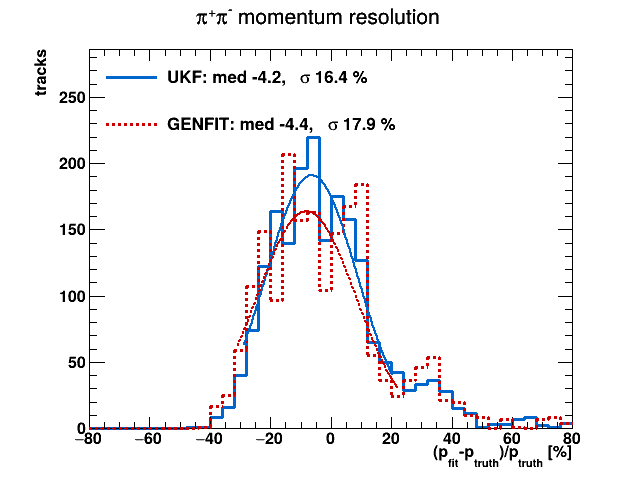
\includegraphics[width=\linewidth]{figs/res_pi_dp.png}\\
{\scriptsize \(\pi^+\pi^-\) momentum residual: both fitters, \(\sigma\sim\)16--18\%.}
\end{columns}
\end{frame}

\begin{frame}{Kalman fits --- examples}
\centering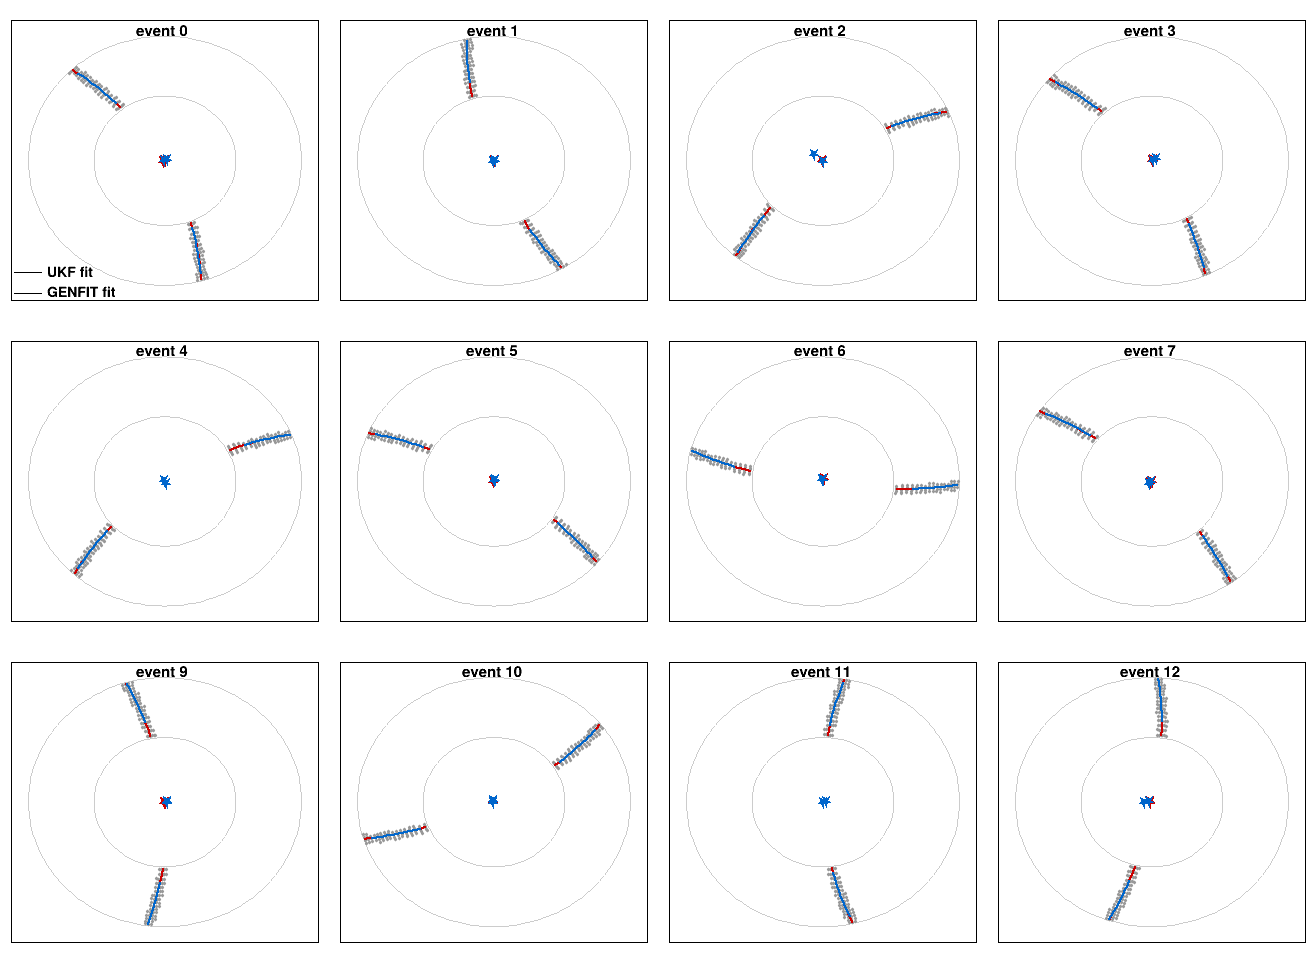
\includegraphics[height=.82\textheight]{figs/fit_examples.png}\\
{\small Twelve events: reconstructed hits (grey) with the \textcolor{blue}{UKF} and \textcolor{red}{GENFIT} fitted trajectories overlaid; the stars are the back-extrapolated vertices (converging on the beam axis at the centre).}
\end{frame}

\begin{frame}{Momentum, angle \& vertex resolution}
\centering
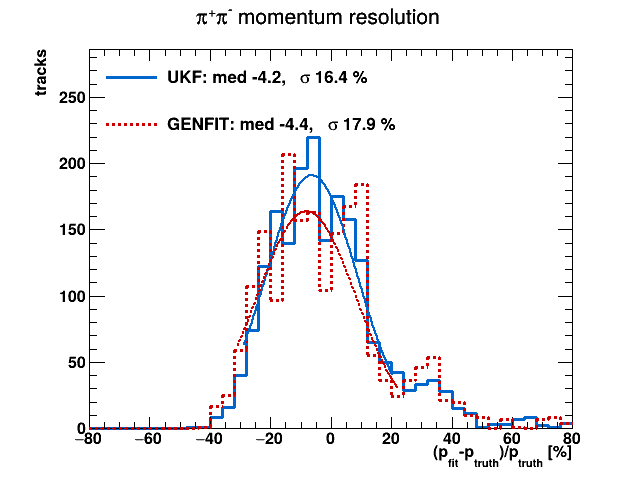
\includegraphics[height=.52\textheight]{figs/res_pi_dp.png}\hfill
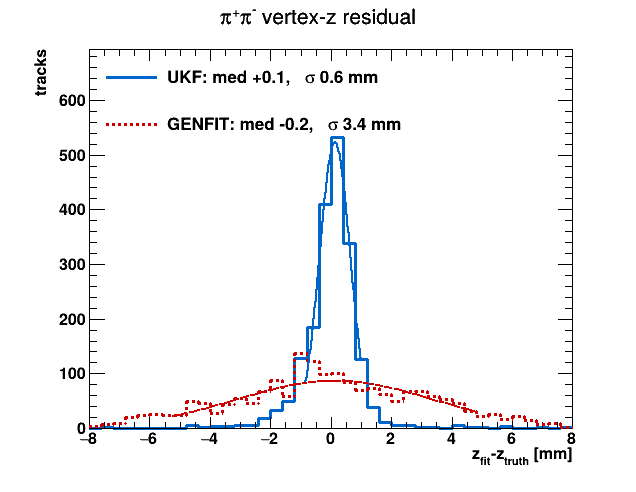
\includegraphics[height=.52\textheight]{figs/res_pi_vz.png}\\[.3em]
{\footnotesize \(\pi^+\pi^-\), 1000 events, identical clusters.\quad
\begin{tabular}{lccccc}\toprule
 & tracking & fitting & momentum \(\sigma\) & \(\theta\) \(\sigma\) & vertex \(\sigma_z\)\\\midrule
UKF & 99.6\% & 99.4\% & \textbf{16\%} & \textbf{2.1}\(^\circ\) & \textbf{0.62} mm\\
GENFIT & 99.6\% & 99.4\% & 18\% & 4.9\(^\circ\) & 3.4 mm\\\bottomrule
\end{tabular}\\ charge-sign \textbf{99.5\%} (both); tracking + fitting efficiency \textbf{$\sim$99.5\%} at 375 MeV/c. UKF wins on angle \& vertex.}
\end{frame}

\begin{frame}{The momentum bias --- and its fix}
\begin{columns}
\column{0.56\textwidth}
\centering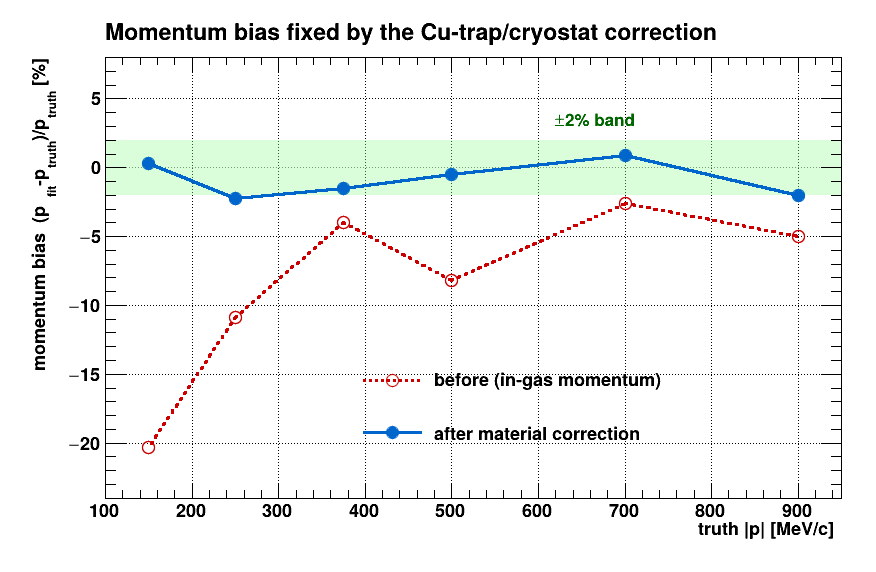
\includegraphics[width=\linewidth]{figs/bias_fix.png}
\column{0.44\textwidth}
Momentum came out biased \emph{low} (\(-\)4\% @375, \(-\)20\% @150 MeV/c). \textbf{Not a reco error} --- the reco measures the in-gas momentum correctly.\\[.4em]
The annihilation vertex sits inside a \textbf{Cu antiproton trap + Al cryostat}; the pion loses \(\sim\)16 MeV escaping to the gas \emph{before} it is tracked (Bethe-Bloch, worse at low \(p\)).\\[.4em]
\textbf{Fix:} a deterministic vertex material correction (both fitters) \(\to\) bias \textbf{within \(\pm\)2\%} across 150--900 MeV/c.
\end{columns}
\end{frame}

\begin{frame}{Particle ID: \(\pi^+\) / \(\pi^-\) separation}
\begin{columns}
\column{0.52\textwidth}
\centering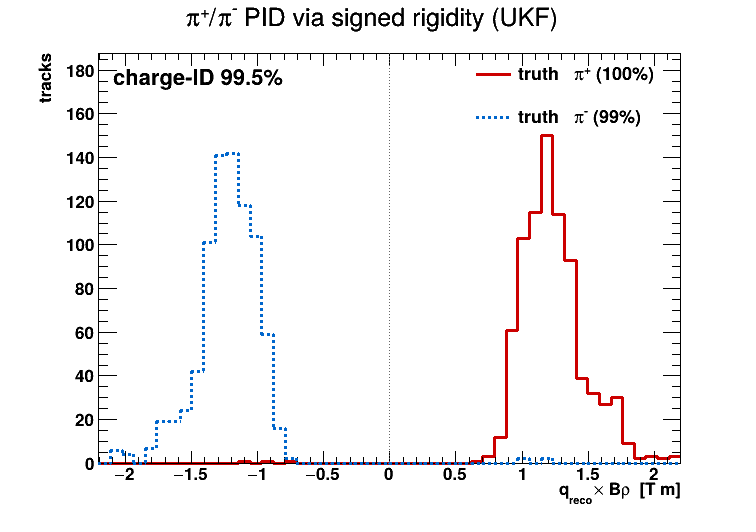
\includegraphics[width=\linewidth]{figs/pid_pipm.png}
\column{0.48\textwidth}
\(\pi^+\) and \(\pi^-\) have \textbf{identical mass} \(\to\) identical dE/dx. They separate purely by \textbf{charge sign} --- the curvature sense in the 4 T field, i.e. signed rigidity \(q\,B\rho = \mathrm{sign}\cdot p/0.2998\) [T\,m].\\[.5em]
Truth-labelled, 1000 events: charge-ID \textbf{99.5\%}, separation power \textbf{S = 5.9\,\(\sigma\)}. The \(\sim\)0.5\% cross-over is the mis-ID.
\end{columns}
\end{frame}

\begin{frame}{Gallery of reconstructed events}
\centering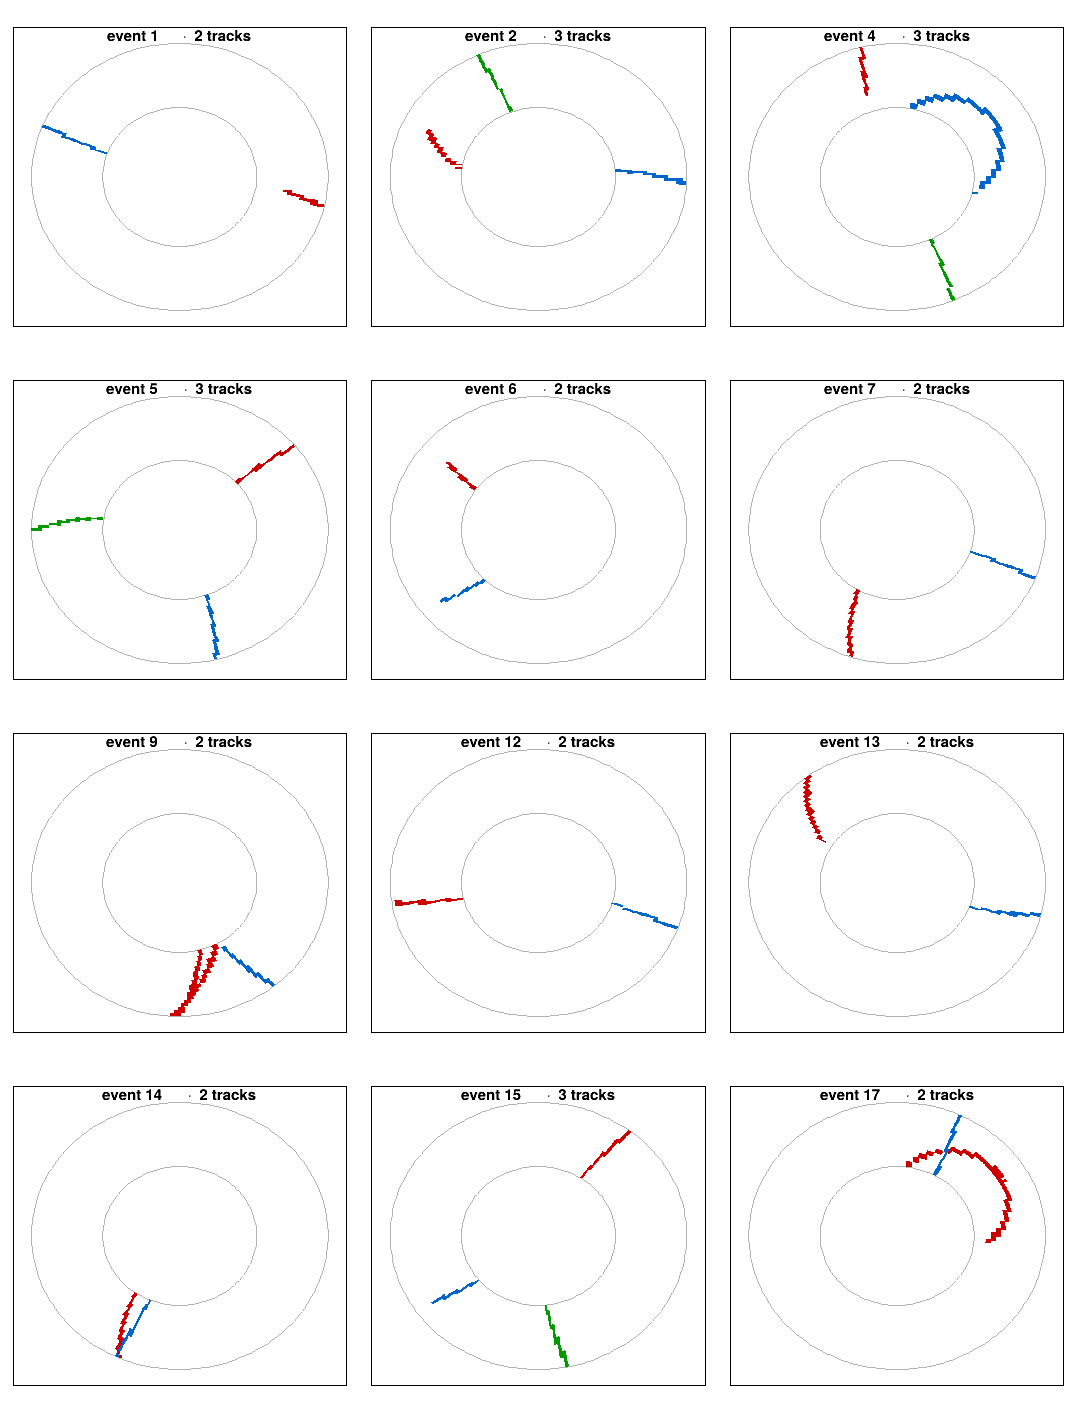
\includegraphics[height=.80\textheight]{figs/gallery.png}\\
{\small Each fired pad as its annular sector, coloured by reconstructed track. 2--3 well-separated tracks per event, various curvatures (momenta).}
\end{frame}

\end{document}
